\documentclass[11pt,a4paper,titlepage]{article}
\usepackage[utf8]{inputenc}
\usepackage[english]{babel}
\usepackage[T1]{fontenc}

\usepackage{float}
\usepackage{graphicx}
\usepackage{setspace}
\usepackage{amsmath}
\usepackage{courier}
\usepackage{amsmath}
\usepackage{listings}
\usepackage{color}
\usepackage[toc, page]{appendix}





\definecolor{mygreen}{rgb}{0,0.6,0}
\definecolor{mygray}{rgb}{0.5,0.5,0.5}
\definecolor{mymauve}{rgb}{0.58,0,0.82}




\lstset{ %
	backgroundcolor=\color{white},   % choose the background color
	basicstyle=\footnotesize,        % size of fonts used for the code
	breaklines=true,                 % automatic line breaking only at whitespace
	captionpos=b,                    % sets the caption-position to bottom
	commentstyle=\color{mygreen},    % comment style
	escapeinside={\%*}{*)},          % if you want to add LaTeX within your code
	keywordstyle=\color{blue},       % keyword style
	stringstyle=\color{mymauve},     % string literal style
}

%\renewcommand{\thesubsection}{\thesection.\alph{subsection}}


\usepackage{booktabs}
\usepackage[backend=biber, bibencoding=utf8, style=ieee]{biblatex}

\addbibresource{references.bib}
\usepackage[final,hidelinks]{hyperref} % must be last package loaded

\author{Ólafur Jón Thoroddsen}  % My name, for the titlepage
\title{\includegraphics{graphics/ru-logo}\\\vspace{10mm}
	Mechatronics II\\T-535-MECH \ \\Homework 4}  % The title, for the titlepage

\begin{document}
	\pagenumbering{arabic}
	\maketitle
	
\section{Homework}

I did not get the delay function to work properly using for loops to waste processor time. I got the blinking working using the hardware timer TCCR1B. Now, the processor runs at 16~MHz, so each clock cycle is $$\text{cs} = \frac{1}{16\cdot 10^{6}} = 6,25\cdot 10^{-8}~\text{s}$$

\noindent To blink the LED at every 10~ms, we use the prescaling of the timer so it only increments the TCNT1 register every 256th clock cycle. This means that between increments, the time that passes is $$256\cdot 6,25\cdot 10^{-8} = 1,6\cdot 10^{-5}~\text{s}$$

\noindent so we need to count up to $$\frac{0,010~\text{s}}{1,6\cdot 10^{-5}} = 625$$

\noindent to get a blink every 10~ms.

The code for this implementation looks like this

\lstinputlisting[language=C, firstline=9,frame=single]{../pwm_diode/main.c}

\noindent The oscilloscope confirms that this results in a very accurate output signal as can be seen on figure~\ref{fig:scope}. The period is 20,05~ms or 0,25\% greater then the theoretical period of 20~ms.

\begin{figure}[h]
	\centering
	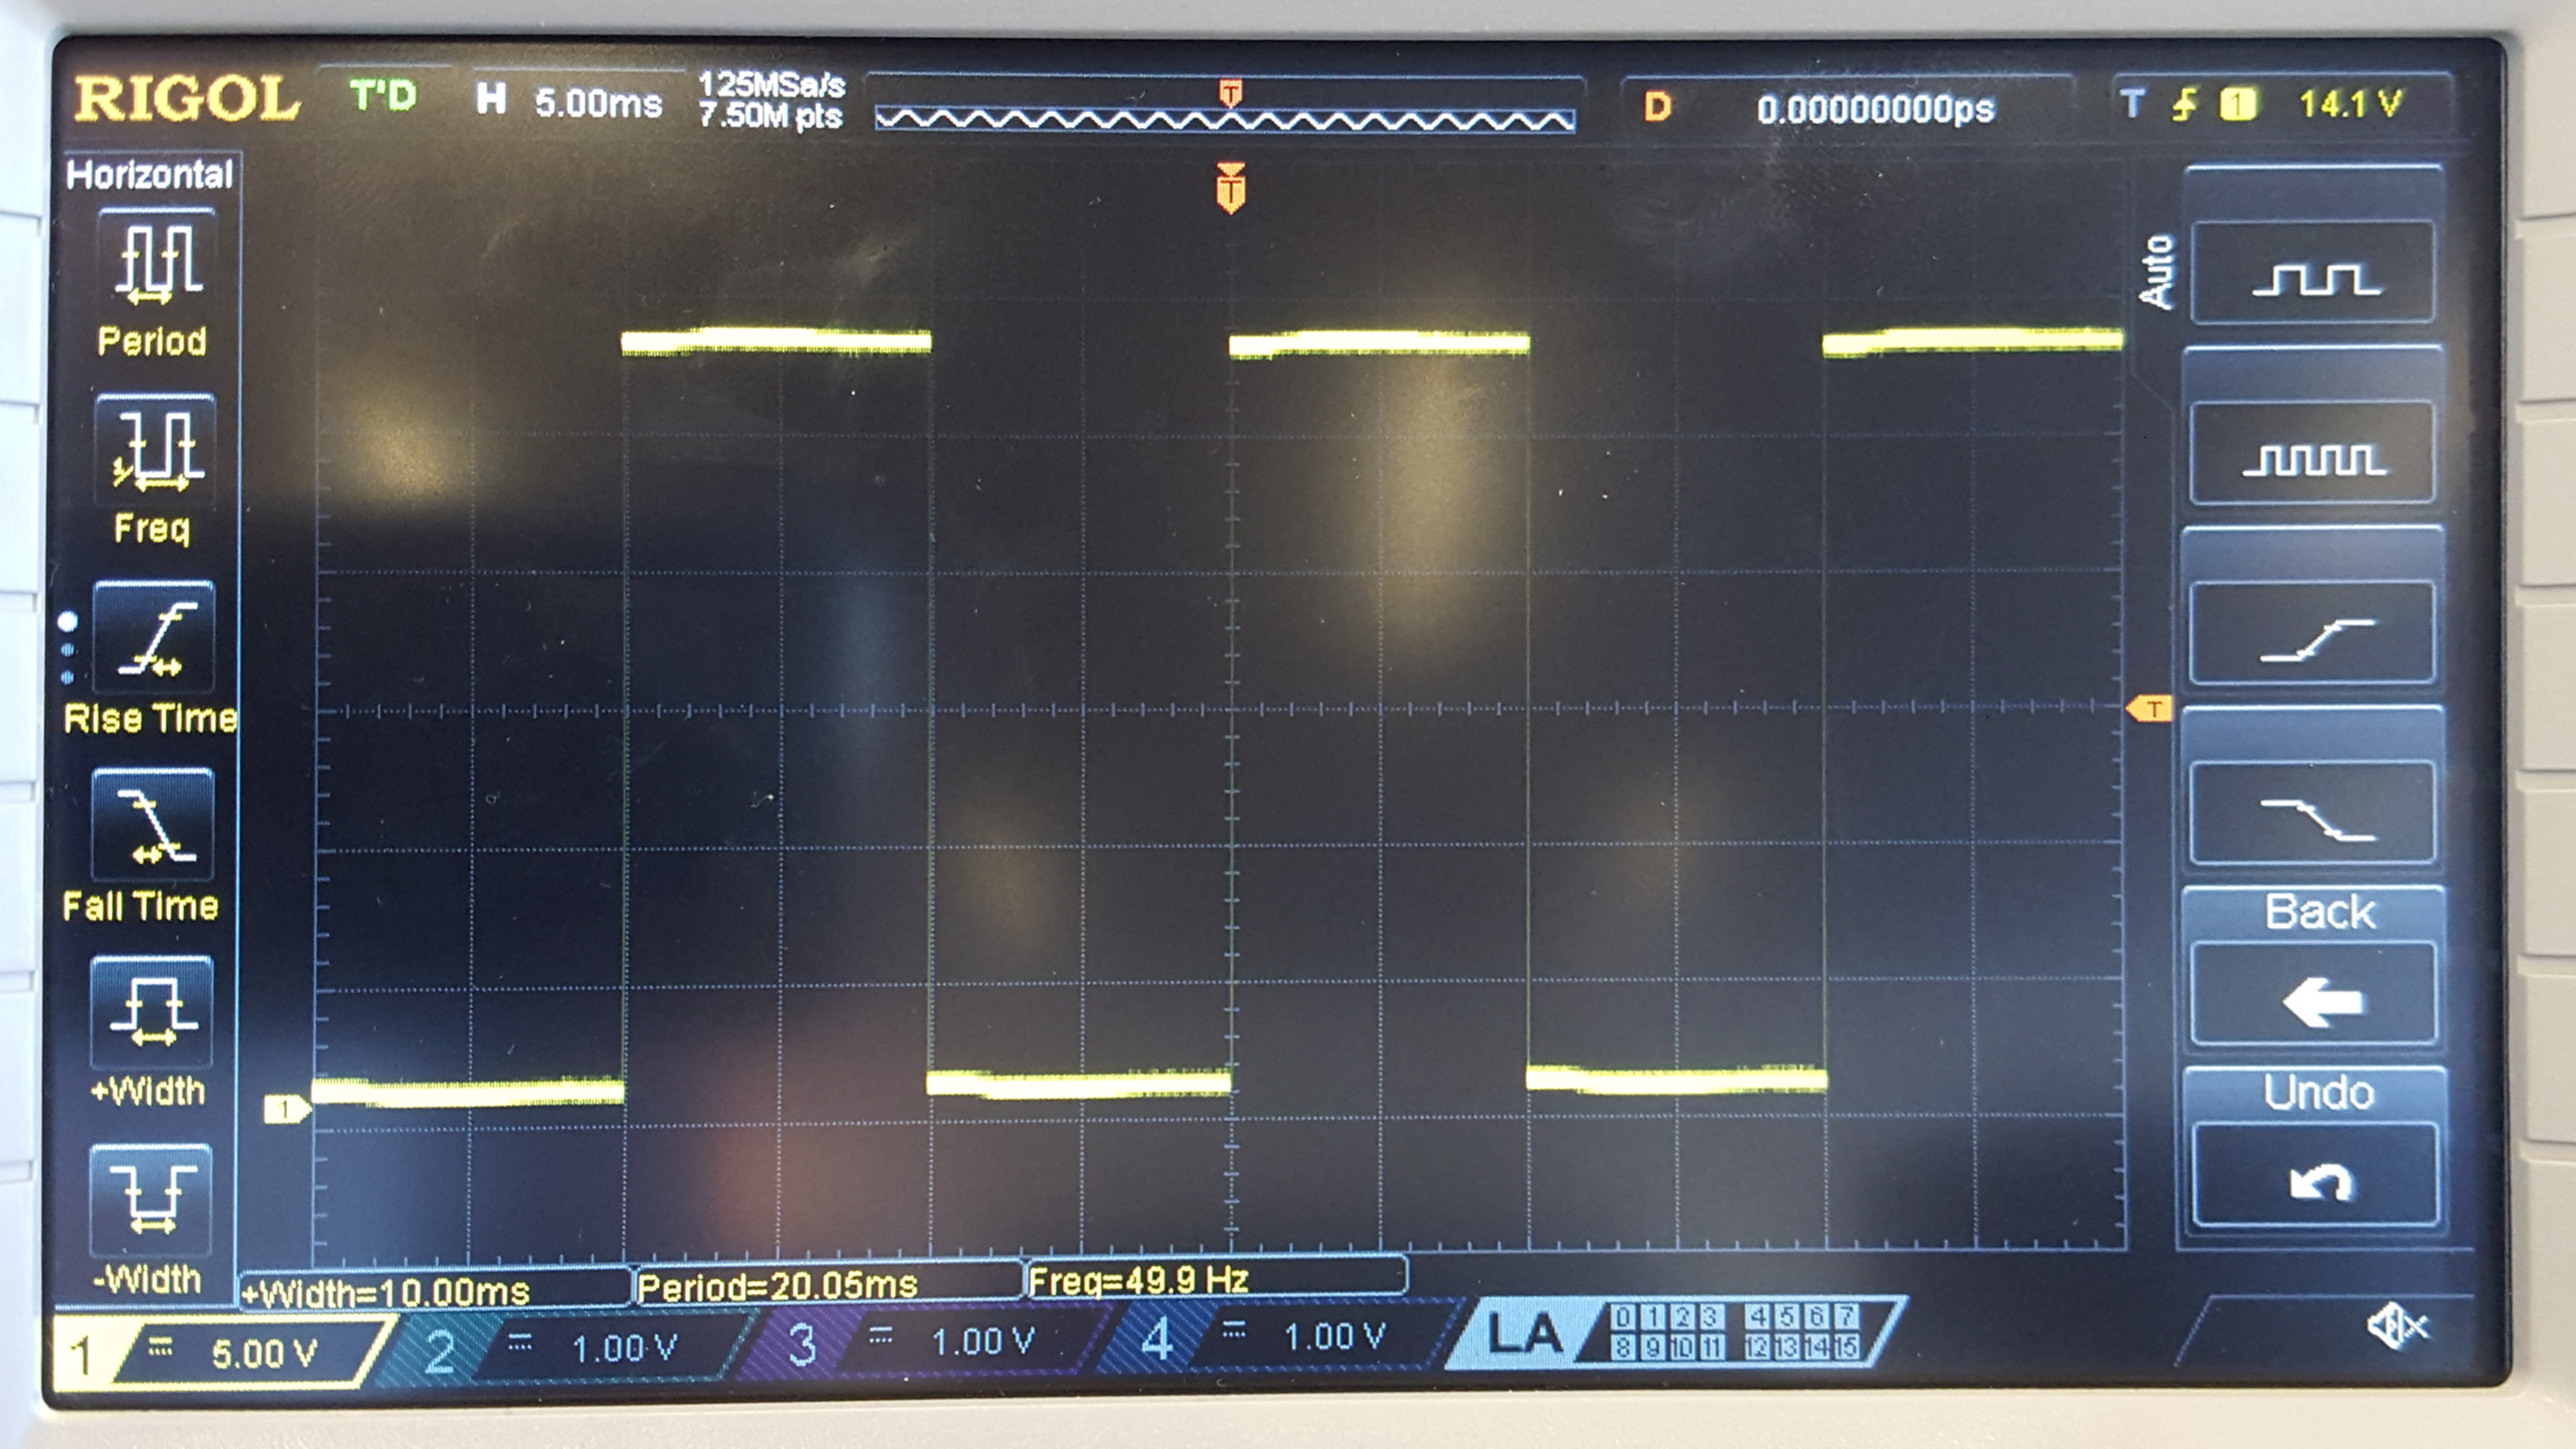
\includegraphics[width=\textwidth]{graphics/socpe}
	\caption{The oscilloscope measurements of the blinking LED}
	\label{fig:scope}
\end{figure}



\end{document}